\documentclass[journal]{IEEEtran}
\usepackage[T1]{fontenc}
\usepackage[utf8]{inputenc}
\usepackage{amsmath,amssymb}
\usepackage{tikz}
\usepackage{booktabs}
\usepackage{url}
\usepackage{cite}

\newcommand{\one}{\mathbf 1}
\newcommand{\T}{\mathsf T}
\newcommand{\erf}{\operatorname{erf}}
\newcommand{\doiline}{DOI: 10.5281/zenodo.24451074}

\markboth{}{}

\begin{document}

\title{The Capacitance of a Cube}

\author{Hrvoje~Abraham and Fable~5.2%
\thanks{Manuscript dated November 23, 2026.}%
\thanks{H. Abraham, e-mail: ahrvoje@gmail.com. Fable 5.2 is a language model of Anthropic.}%
\thanks{The programs are at \protect\url{https://github.com/ahrvoje/blog}, folder \texttt{cube}. \doiline.}}

\maketitle

\begin{abstract}
The electrostatic capacitance of a metal cube has no known closed form. This paper gives two results. The first is an infinite series of positive terms for the capacitance, made of uniformly charged spherical shells. Each term is an algebraic number that follows from a closed formula and a recursion, with no integral. The series is exact, but too slow to give many decimals. The second is a fast series of the same structure, made of polynomial charge patches on the faces, graded toward the edges. All its integrals reduce to the error function. It gives the capacitance of a cube of side $s$ as $4\pi\varepsilon_0 s\kappa$ with $\kappa = 0.660\,678\,154\,099\,568\,000 \pm 10^{-18}$. The error is an estimate from the observed convergence, not a proved bound.
\end{abstract}

\begin{IEEEkeywords}
Capacitance, cube, variational method, method of moments, boundary elements, Cholesky factorization, series acceleration.
\end{IEEEkeywords}

\section{Introduction}
\IEEEPARstart{A}{metal} sphere of radius $r$ has the capacitance $4\pi\varepsilon_0 r$. For a metal cube no formula is known, only numbers. The best published value has 13 digits \cite{helsing}.

This paper has two results. The first is a series of positive terms for that number, made of charged spherical shells. Each term is an algebraic number from a closed formula, with no integral. The series is exact, but too slow to give many decimals. The second is a fast series of the same structure, made of charged patches on the faces. It gives
\begin{equation}
C_{\text{cube}} = 4\pi\varepsilon_0\, s\,\kappa, \quad \kappa = 0.660\,678\,154\,099\,568\,000 \pm 10^{-18}
\label{eq:result}
\end{equation}
for a cube of side $s$. The error is an estimate from the convergence, not a proved bound.

\section{The Problem}
Put the unit cube $K$ at potential 1, in units where the potential of a point charge $q$ at distance $r$ is $q/r$. The charge moves to the surface and settles in an equilibrium distribution $\mu$. Its total is the number $\kappa$. In these units a sphere of radius $r$ holds the charge $r$, so $\kappa$ is the radius of the sphere that is equivalent to the cube.

The density of $\mu$ is not known. It is infinite along the edges and still stronger at the corners, and this is the full difficulty of the problem.

One classical fact makes the problem approachable without the density \cite{polya}. Take any charge distribution $\nu$ in the cube, not necessarily in equilibrium, with total charge $q(\nu)$ and energy
\begin{equation}
E(\nu) = \iint \frac{d\nu(x)\, d\nu(y)}{|x-y|}.
\end{equation}
Then
\begin{equation}
2\,q(\nu) - E(\nu) = \kappa - E(\mu - \nu) \le \kappa .
\label{eq:principle}
\end{equation}
The proof is one line. The potential of $\mu$ is 1 on the whole cube, thus the mutual energy of $\mu$ and $\nu$ is $q(\nu)$, and $E(\mu-\nu) = \kappa - 2q(\nu) + E(\nu)$ cannot be negative. Each guess $\nu$ gives a lower bound for $\kappa$, and the error of the bound is the energy of the error of the guess. A guess with an error of $10^{-8}$ gives $\kappa$ to $10^{-16}$.

Now take $N$ fixed distributions $\sigma_1,\dots,\sigma_N$ of unit charge and let the guess be $\nu = \sum q_j \sigma_j$. The best charges $q_j$ follow from the linear system $Gq = \one$, and the bound becomes
\begin{equation}
\kappa_N = \one^{\T} G^{-1} \one \le \kappa, \qquad G_{ij} = E(\sigma_i, \sigma_j).
\label{eq:bound}
\end{equation}

The system has a physical meaning. The product $(Gq)_i$ is the potential of all the trial charges, averaged over $\sigma_i$. Thus $Gq = \one$ says: the potential is 1 on each $\sigma_i$ on average. This is the conductor condition, as far as the family can test it. The bound $\one^{\T} G^{-1} \one = \sum q_j$ is the total charge that does this. In Maxwell's words \cite{maxwell}, $G$ is the matrix of the coefficients of potential, and the sum of all entries of its inverse is the capacitance of the parts joined together.

All that is necessary is a family $\sigma_j$ for which the energies $G_{ij}$ are easy.

\section{The Shell Series}
The easiest family is a uniformly charged spherical shell. By Newton's shell theorem, a shell of radius $R$ and unit charge has the potential $1/\max(R, d)$ at distance $d$ from its centre: outside it is a point charge, inside the potential is constant. The energy of two shells of radii $R$ and $S$, with centres at distance $d$, is then elementary:
\begin{equation}
\small
G(R,S,d)=
\begin{cases}
\dfrac{1}{\max(R,S)}, & d \le |R-S|,\\[8pt]
\dfrac{1}{d}\Big(1-\dfrac{(R+S-d)^2}{4RS}\Big), & |R-S| < d < R+S,\\[8pt]
\dfrac{1}{d}, & d \ge R+S.
\end{cases}
\label{eq:shell}
\end{equation}
The three cases are: one shell inside the other, partial overlap, and shells apart.

For the family, divide the cube into $n^3$ cells and put one shell into each cell, of radius $1/2n$. Do this for $n = 1, 2, 4, 8, \dots$ and keep all the shells of all the grids (Fig.~\ref{fig:shells}, left).

\begin{figure}[!t]
\centering
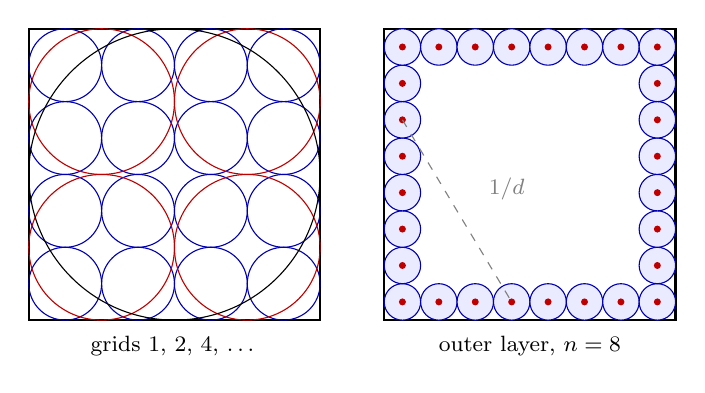
\begin{tikzpicture}[scale=3.7]
% nested shells
\draw[thick] (0,0) rectangle (1,1);
\foreach \i in {0,...,3} \foreach \j in {0,...,3}
  \draw[blue!70!black] ({(2*\i+1)/8},{(2*\j+1)/8}) circle (1/8);
\foreach \i in {0,1} \foreach \j in {0,1}
  \draw[red!75!black] ({(2*\i+1)/4},{(2*\j+1)/4}) circle (1/4);
\draw (0.5,0.5) circle (0.5);
\node[below, font=\footnotesize] at (0.5,-0.02) {grids 1, 2, 4, \dots};
% boundary shells
\begin{scope}[xshift=1.22cm]
\draw[thick] (0,0) rectangle (1,1);
\foreach \i in {0,...,7} \foreach \j in {0,...,7} {
  \pgfmathtruncatemacro{\edge}{(\i==0 || \i==7 || \j==0 || \j==7) ? 1 : 0}
  \ifnum\edge=1
    \draw[blue!70!black, fill=blue!8] ({(2*\i+1)/16},{(2*\j+1)/16}) circle (1/16);
    \fill[red!75!black] ({(2*\i+1)/16},{(2*\j+1)/16}) circle (0.012);
  \fi
}
\draw[dashed, gray] (1/16,11/16) -- (7/16,1/16);
\node[gray, font=\footnotesize] at (0.42,0.45) {$1/d$};
\node[below, font=\footnotesize] at (0.5,-0.02) {outer layer, $n = 8$};
\end{scope}
\end{tikzpicture}
\caption{Trial charges in a cross-section of the cube. Left: the nested family that gives the series; each new shell adds one term. Right: the cheaper family that keeps only the shells next to the surface. From outside, a shell acts as a point charge at its centre.}
\label{fig:shells}
\end{figure}

Order the shells by grid, and in a grid by position. The matrix $G$ of the first $N$ shells is the top left corner of the matrix of the first $N+1$ shells. Its Cholesky factor $G = LL^{\T}$ has the same property, and with $z = L^{-1}\one$
\begin{equation}
\kappa_N = \one^{\T} G^{-1} \one = \lVert L^{-1}\one\rVert^2 = \sum_{j<N} z_j^2,
\quad
\kappa = \sum_{j=0}^{\infty} z_j^2 .
\label{eq:series}
\end{equation}
Each new shell adds one term. The term is not negative, and the terms before it do not change.

The three objects have a simple meaning. $G$ holds the energies of the shells. $L$ makes the shells independent: it is the Gram--Schmidt process with the energy as the scalar product, and it replaces the shells one by one with charge distributions $e_0, e_1, \dots$ that have unit energy and zero mutual energy. The number $z_j$ is the total charge of $e_j$. The series is then Parseval's identity: the equilibrium charge is $\sum z_j e_j$, and its energy $\kappa$ is $\sum z_j^2$.

The series is also a recursion. Shell $n$ needs its energies $G_{nj}$ with the shells before it and the rows of $L$ before it:
\begin{align}
L_{nj} &= \frac{1}{L_{jj}}\Big(G_{nj} - \sum_{k<j} L_{nk} L_{jk}\Big), \quad j < n, \label{eq:rec1}\\
L_{nn}^2 &= G_{nn} - \sum_{k<n} L_{nk}^2, \label{eq:rec2}\\
z_n &= \frac{1}{L_{nn}}\Big(1 - \sum_{k<n} L_{nk}\, z_k\Big). \label{eq:rec3}
\end{align}
The sum in \eqref{eq:rec3} is the potential of the best charge so far, averaged over the new shell, so the numerator is what the potential there still lacks to 1. $L_{nn}^2$ is the energy of the part of the new shell that the earlier shells cannot imitate. The new term $z_n^2$ is the square of the first divided by the second. The recursion keeps all earlier rows: term $n$ costs about $n^2$ operations.

By hand, for the first two shells: the inscribed sphere has $G_{00} = 1/R = 2$, thus $L_{00} = \sqrt2$ and $z_0 = 1/\sqrt2$. The second shell has the radius $\frac14$ and the distance $\frac{\sqrt3}{4}$ to the first one. They overlap, and \eqref{eq:shell} gives $G_{10} = 3 - 2/\sqrt3$ and $G_{11} = 4$. Then $L_{10} = G_{10}/\sqrt2$, $L_{11}^2 = 4 - G_{10}^2/2 = 2\sqrt3 - \frac76$ and $z_1 = (1 - G_{10}/2)/L_{11}$.

The centres and radii are rational, the distances are square roots of rationals, and the recursion needs only arithmetic and square roots, so each $z_j$ is an algebraic number. The first two are
\begin{equation}
z_0^2 = \frac12, \qquad z_1^2 = \frac{\left(\frac1{\sqrt3}-\frac12\right)^2}{2\sqrt3-\frac76} = 0.002604\ldots
\end{equation}
The first term is the sphere inscribed in the cube. Table~\ref{tab:cumulative} gives the partial sums at the end of each grid. The series is exact and its terms are explicit, but eight times more terms halve the error. Twenty digits would need about $10^{59}$ terms.

\begin{table}[!t]
\caption{Partial Sums of the Shell Series}
\label{tab:cumulative}
\centering
\begin{tabular}{rrll}
\toprule
Grid & Terms & Partial sum & Error\\
\midrule
1 & 1 & 0.500000000 & 0.16\\
2 & 9 & 0.526938289 & 0.13\\
4 & 73 & 0.586840900 & 0.074\\
8 & 585 & 0.620510985 & 0.040\\
16 & 4\,681 & 0.639356611 & 0.021\\
32 & 37\,449 & 0.649547183 & 0.011\\
64 & 299\,593 & 0.654930553 & 0.0057\\
\bottomrule
\end{tabular}
\end{table}

\section{Why the Shell Series Is Slow}
The charge is on the surface, so the shells deep in the cube do little. Keep only the outer layer of one grid (Fig.~\ref{fig:shells}, right). These shells have equal radii and do not overlap, and the matrix becomes very simple:
\begin{equation}
Q_n = \frac1n\, \one^{\T} M^{-1} \one, \quad M_{kk} = 2, \quad M_{k\ell} = \frac{1}{|k-\ell|},
\end{equation}
where $k$ and $\ell$ are the integer positions of the cells. The cube has 48 symmetries, so the system has one unknown for each orbit of cells: 8\,256 unknowns for the 390\,152 shells of $n = 256$. Table~\ref{tab:boundary} gives the values.

\begin{table}[!t]
\caption{Boundary Shells}
\label{tab:boundary}
\centering
\begin{tabular}{rrll}
\toprule
$n$ & Shells & $Q_n$ & Error\\
\midrule
16 & 1\,352 & 0.638074892611 & 0.023\\
32 & 5\,768 & 0.648744830566 & 0.012\\
64 & 23\,816 & 0.654459967974 & 0.0062\\
128 & 96\,776 & 0.657468745801 & 0.0032\\
256 & 390\,152 & 0.659033442870 & 0.0016\\
512 & 1\,566\,728 & 0.659839854768 & 0.00084\\
\bottomrule
\end{tabular}
\end{table}

The error is close to $0.43/n$. Richardson extrapolation removes an error term $c\,n^{-p}$ from two values, $(2^p Q_{2n} - Q_n)/(2^p-1)$. The data show the powers $1$ and $4/3$ clearly, and then the powers come close to each other. With the powers $1, 4/3, 5/3, 2$ the values up to $n = 256$ give $0.66067827$, with an error of $1.2\cdot10^{-7}$, and up to $n = 512$ the error is $3\cdot10^{-8}$. More powers gave 8 digits, not more.

The reason is the edges. Near an edge the density grows like $d^{-1/3}$, where $d$ is the distance to the edge, and at a corner it grows faster, with an irrational power. Each of these adds its own sequence of fractional powers of $1/n$ to the error. A sphere has the same size in all directions. To follow the density at distance $d$ from an edge, the shells there must have a radius near $d$, and then $1/d$ of them are necessary along the edge. No arrangement of shells escapes this count.

\section{Patches}
The cure is to let the trial charges become thin. Put the charge on the faces, on rectangular patches that are a fixed fraction of the neighbour patch in the direction of each edge (Fig.~\ref{fig:patches}). Twenty-three layers reach from the centre of a face to $10^{-13}$ from the edge. On each patch the density is a polynomial, of a higher degree on the large patches in the middle and of a low degree on the small ones near the edges.

\begin{figure}[!t]
\centering
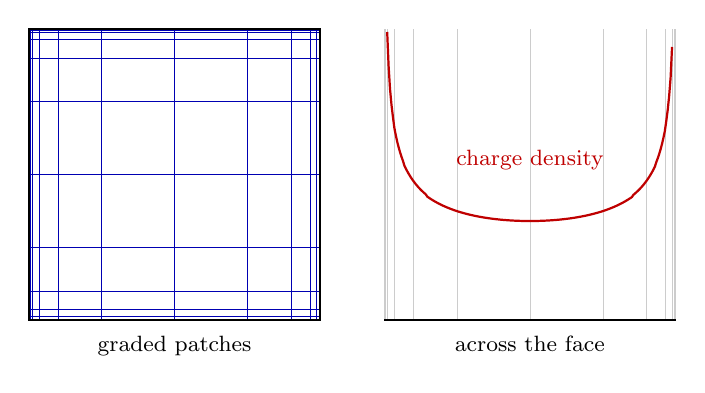
\begin{tikzpicture}[scale=3.7]
\def\nodes{0,0.2503,0.4002,0.4645,0.4879,0.4959,0.4986,0.5}
\foreach \v in \nodes {
  \draw[blue!70!black, very thin] ({0.5+\v},0) -- ({0.5+\v},1);
  \draw[blue!70!black, very thin] ({0.5-\v},0) -- ({0.5-\v},1);
  \draw[blue!70!black, very thin] (0,{0.5+\v}) -- (1,{0.5+\v});
  \draw[blue!70!black, very thin] (0,{0.5-\v}) -- (1,{0.5-\v});
}
\draw[thick] (0,0) rectangle (1,1);
\node[below, font=\footnotesize] at (0.5,-0.02) {graded patches};
\begin{scope}[xshift=1.22cm]
\foreach \v in \nodes {
  \draw[gray!40, very thin] ({0.5+\v},0) -- ({0.5+\v},1);
  \draw[gray!40, very thin] ({0.5-\v},0) -- ({0.5-\v},1);
}
\draw[thick] (0,0) -- (1,0);
\draw[red!75!black, thick, domain=-0.4898:0.4898, samples=200]
  plot ({0.5+\x},{0.2143*(0.25-\x*\x)^(-1/3)});
\node[red!75!black, font=\footnotesize] at (0.5,0.55) {charge density};
\node[below, font=\footnotesize] at (0.5,-0.02) {across the face};
\end{scope}
\end{tikzpicture}
\caption{The fast family. Left: one face, with patches graded toward the edges. Each layer is a fixed fraction of the layer before it. Right: the density across the face, which grows like $d^{-1/3}$ at the edges.}
\label{fig:patches}
\end{figure}

The energies of two patches are fourfold integrals of $1/r$, and they must be accurate to all digits. One identity makes them easy \cite{stenger,beylkin}:
\begin{equation}
\frac1r = \frac{2}{\sqrt\pi}\int_0^\infty e^{-t^2 r^2}\,dt \approx \sum_k w_k\, e^{-t_k^2 r^2}.
\label{eq:gauss}
\end{equation}
With $t = e^u$ the integrand is smooth and decreases fast in both directions, and the plain trapezoidal rule with a step $h$ in $u$ is enough. Its relative error is the same for all distances $r$. The Fourier transform of the integrand is a gamma function, and this gives the bound $2\sqrt2\, e^{-\pi^2/2h}$. The step $h = 0.12$ is the largest round step with a bound below the target: $4\cdot10^{-18}$. The work grows like $1/h$, so a smaller step only costs time. The measured error is smaller than the bound, because it changes sign with $\ln r$ and averages out: the steps $0.2$, $0.15$ and $0.12$ move $\kappa$ by $2\cdot10^{-13}$, $8\cdot10^{-17}$ and $5\cdot10^{-22}$.

A Gaussian of $r$ is a product of Gaussians of the coordinates. Thus each energy is a sum of products of integrals in one variable,
\begin{equation}
\iint p(x)\, q(x')\, e^{-t^2 (x-x')^2}\, dx\, dx',
\end{equation}
with polynomials $p$ and $q$ on two intervals. The polynomials are not unknowns. They are fixed before the calculation: the Legendre polynomials $P_0, P_1, \dots$ up to the chosen degree, each moved to one interval of the mesh. Only the amount of charge on each of them is unknown.

Integration by parts moves all derivatives to the polynomials, and what stays are repeated integrals of the Gaussian at the differences of the interval ends. These are combinations of $\erf$ and $\exp$. Again there is no numerical integration over the cube.

\section{The Recipe}
The full construction has four steps. All formulas are explicit.

\subsection{The Gaussians}
Take $t_k = e^{0.12\,k}$ and $w_k = \frac{2}{\sqrt\pi}\, 0.12\, t_k$ for $k = -350, \dots, 366$.

\subsection{One Edge}
Choose functions $\varphi_1, \dots, \varphi_N$ of one variable on the edge $[-\frac12, \frac12]$. Here each is a Legendre polynomial on one interval of the mesh, and zero outside it. With the mesh nodes $x_0 < x_1 < \dots$ and the interval $[x_i, x_{i+1}]$ of length $h_i$, the function of degree $n$ on this interval is
\begin{equation}
\varphi_{i,n}(x) = \frac{1}{h_i}\, P_n(\xi), \qquad \xi = \frac{2x - x_i - x_{i+1}}{h_i},
\end{equation}
where $P_0 = 1$, $P_1 = \xi$, $P_2 = \frac12(3\xi^2 - 1)$, and so on. The variable $\xi$ stretches the interval to $[-1, 1]$, where the Legendre polynomials live. The index $a$ counts the pairs $(i, n)$. The function of degree 0 is the uniform charge 1 on the interval. The higher degrees have the total charge 0, because $\int_{-1}^{1} P_n = 0$ for $n \ge 1$: they only move charge inside the interval, as a slope, a curvature, and so on.

The nodes are $x_i = \pm\frac12 \tanh(16\, i/I)$ for $I$ layers on each half of the edge, and the last node is the end of the edge. The distance of a node to the edge is $\frac12 - \frac12\tanh u = 1/(1 + e^{2u})$, which is $e^{-2u}$ for large $u$. Equal steps in $u$ thus give distances in a fixed ratio, $e^{-32/I}$ from one node to the next. The density near an edge is a power, $d^{-1/3}$, and a power looks the same at each scale. So each scale needs the same number of intervals, and that is a mesh with a fixed ratio. In the middle of the face the density is smooth, and there $\tanh u \approx u$ gives nearly equal intervals. The function $\tanh$ is a convenient choice, not a necessary one. The number 16 sets the smallest interval, $e^{-32}$. The density is the same on both halves of the edge, so the program uses each function together with its mirror image, $\varphi(x) + \varphi(-x)$, as one function.

For each $t = t_k$ make two tables and note the charges:
\begin{align}
A_{ac} &= \iint \varphi_a(x)\, \varphi_c(x')\, e^{-t^2 (x-x')^2}\, dx\, dx', \\
s_a &= \int \varphi_a(y)\, e^{-t^2 (1/2-y)^2}\, dy, \\
m_a &= \int \varphi_a(y)\, dy .
\end{align}

\subsection{One Face}
The trial charges on a face are the products $\varphi_a(x)\,\varphi_b(y)$, and the density is $\sum C_{ab}\, \varphi_a(x)\, \varphi_b(y)$. The numbers $C_{ab}$ are the only unknowns. All six faces carry the same density. The energy of the product $(a,b)$ on one face with the product $(c,d)$ on all six faces is
\begin{multline}
H_{ab,cd} = \sum_k w_k \Big[ \big(1 + e^{-t_k^2}\big) A_{ac} A_{bd} \\
+ 2\, A_{ac}\, s_b\, s_d + 2\, s_a\, A_{bc}\, s_d \Big].
\label{eq:H}
\end{multline}
The first term is the face itself and the opposite face, at distance 1. The other two are the four adjacent faces.

\subsection{The System}
Solve $H C = m$, where $m_{ab} = m_a m_b$. Then $\kappa_N = 6\, m^{\T} C$.

\subsection{The Smallest Case, Almost by Hand}
Take one function, $\varphi = 1$ on the full edge: a uniformly charged cube. The two tables are
\begin{equation}
A(t) = \frac{\sqrt\pi\, t\, \erf t + e^{-t^2} - 1}{t^2}, \qquad s(t) = \frac{\sqrt\pi\, \erf t}{2t},
\end{equation}
for example $A(1) = 0.861528$ and $s(1) = 0.746824$. The system is one equation, and
\begin{align}
h &= \sum_k w_k \Big[ \big(1 + e^{-t_k^2}\big) A(t_k)^2 + 4\, A(t_k)\, s(t_k)^2 \Big] \nonumber\\
  &= 9.2475851, \\
\kappa_1 &= \frac6h = 0.648818 .
\end{align}
A coarse sum with the step $0.5$ and 33 terms, from $t = e^{-8}$ to $e^{8}$, already gives $0.6490$. So the first term of the fast series is $0.6488$, where the first term of the shell series was $0.5$. Each further function $\varphi$ adds rows to $H$ and terms to the series, by the same four steps.

\section{How the System Is Solved}
Why $HC = m$? It is the same statement as $Gq = \one$ for the shells. Add a small charge $\delta$ of the shape $\varphi_a\varphi_b$ to the faces. The bound $2q - E$ changes in proportion to $\delta\,(m_{ab} - (HC)_{ab})$, and at the best $C$ no such change can help, so all these differences are zero.

Physically, $(HC)_{ab}$ is the potential of the full trial charge on a face, weighted with $\varphi_a\varphi_b$ and integrated, and $m_{ab}$ is the same integral of the potential 1. So the system says: the surface is at potential 1, as far as the trial functions can test it. For the functions of degree 0 this means that the mean potential over each patch is exactly 1. The higher degrees also remove its mean slope and curvature over the patch. A conductor has the potential 1 at every point of its surface. The system asks for this in as many ways as there are unknowns.

The matrix $H$ is symmetric and positive definite, and it is full: each patch acts on each other patch. The density must not change when $x$ and $y$ change places, so $C_{ab} = C_{ba}$, and $N$ functions on the edge give $N(N+1)/2$ unknowns. The largest run has $N = 343$ and 58\,996 unknowns.

The solution has three stages.
\begin{enumerate}
\item Scale $H$ to a unit diagonal, because the energies of the small patches near the edges are much larger than the energies of the large ones.
\item Factor $H = LL^{\T}$ with Cholesky in double precision, and solve $Lz = m$. Then
\begin{equation}
\kappa_N = 6\, m^{\T} H^{-1} m = 6 \sum_j z_j^2 .
\end{equation}
\item Refine. Double precision gives $\kappa_N$ to about $10^{-16}$, and the last digits need more. Compute the residual $m - HC$ in double-double arithmetic (31 digits), solve for the correction with the same factor $L$, and add it. Two rounds bring the residual to $10^{-30}$.
\end{enumerate}

The residual does not need the matrix $H$ in high precision. With the tables as matrices, the product $HC$ for one Gaussian is $(1 + e^{-t^2})\,A C A + 2\,(A C s)\,s^{\T} + 2\,s\,(A C s)^{\T}$, three small matrix products. As with the shells, the result is a lower bound and a sum of positive terms, one term for each trial function.

\section{Results}
Table~\ref{tab:patches} gives the convergence. Each row is a lower bound. The errors are differences from the last row, and they fall by a factor of 100 to 2000 from row to row. Sixteen digits need about 17\,000 unknowns. The shells gave 3 digits with 1.5 million.

\begin{table}[!t]
\caption{Patches: Layers, Top Degree, Unknowns, Lower Bound, Error and Time}
\label{tab:patches}
\centering
\footnotesize
\setlength{\tabcolsep}{3pt}
\begin{tabular}{rrrllr}
\toprule
$I$ & Deg. & Unkn. & $\kappa_N$ & $\kappa-\kappa_N$ & Time, s\\
\midrule
8 & 2 & 190 & 0.660605384086 & $7\cdot10^{-5}$ & 6\\
12 & 4 & 903 & 0.660678004068 & $1.5\cdot10^{-7}$ & 14\\
16 & 6 & 2\,701 & 0.660678153932361 & $2\cdot10^{-10}$ & 30\\
20 & 8 & 6\,328 & 0.660678154099484426 & $8\cdot10^{-14}$ & 59\\
23 & 10 & 16\,653 & 0.660678154099567955 & $4\cdot10^{-17}$ & 159\\
23 & 12 & 19\,503 & 0.660678154099567999066 & $3\cdot10^{-19}$ & 203\\
32 & 14 & 58\,996 & 0.660678154099567999411 & & 1\,123\\
\bottomrule
\end{tabular}
\end{table}

The result is \eqref{eq:result}. The best run gives $0.660\,678\,154\,099\,567\,999\,4$, a lower bound. The last two runs differ by $3.5\cdot10^{-19}$, and the step before that was $4\cdot10^{-17}$, so the next step is far below $10^{-19}$. The numerical parameters add at most $3\cdot10^{-19}$ each. From these we assume an error of $10^{-18}$. It is an estimate, not a proved bound. The nearest double is 0.660678154099568.

Three numerical parameters could spoil the last digits, and each of them was varied.
\begin{itemize}
\item The smallest patch. The mesh stops at $e^{-32}$ from the edge. With two more layers the result moves by $2\cdot10^{-19}$.
\item The step of the Gaussian sum. The steps $0.12$ and $0.10$ agree to $5\cdot10^{-22}$. The nodes $t_k$ must be exact: when $\ln t_k$ was rounded to double precision, the result moved by $2\cdot10^{-17}$.
\item The range of the Gaussian sum, $e^{-42} \le t \le e^{44}$. A wider range moves the result by less than $3\cdot10^{-19}$.
\end{itemize}
The value agrees with the best published one, $0.66067815409957$ \cite{helsing}, in all its digits.

\section{The Programs}
Both programs are plain Julia with threads, without packages. The program \texttt{shells.jl} makes Tables~\ref{tab:cumulative} and \ref{tab:boundary}. The matrix is assembled over the orbits of the 48 symmetries. The values $Q_n$ are refined to 28 digits with double-double residuals, so that the extrapolation does not amplify rounding errors. The program \texttt{patches.jl} makes Table~\ref{tab:patches}. The integrals in one variable cancel strongly and use 1024-bit numbers. The matrix $H$ and its Cholesky factor are in double precision, and the solution is refined with double-double residuals.

On a 32-thread desktop (Core i9-13900K, 64~GB) the shell tables take about 2 minutes, most of it for $n = 512$, and the first six rows of Table~\ref{tab:patches} take 8 minutes. The last row needs 19 minutes and about 30~GB.

\section{Prior Art}
Is this new? The idea is not. It is the Rayleigh--Ritz method: restrict a variational problem to a finite family and solve a linear system. Each part has a name and a history.

The energy principle \eqref{eq:principle} is due to Gauss and Thomson; for the capacity it is the base of \cite{polya}. A finite family with the matrix of energies is Maxwell's method of subareas \cite{maxwell}, in electrical engineering the method of moments \cite{harrington}, and with the energy as the scalar product the Galerkin boundary element method. The formula \eqref{eq:bound} with its error identity is in \cite{betcke}. The energy \eqref{eq:shell} of two overlapping shells is, up to a factor, the trace of the Rotne--Prager--Yamakawa tensor of hydrodynamics \cite{zuk}; there the same sum over the inverse matrix gives the hydrodynamic radius of a chain of beads. The series \eqref{eq:series} is Cholesky, Gram--Schmidt and Parseval. Patches graded in a fixed ratio toward the edges, with polynomials on them, are the $hp$ boundary element method, which is known to converge exponentially for such densities. The sum of Gaussians \eqref{eq:gauss} is a standard tool as well \cite{stenger,beylkin}.

What can be particular to this paper is the combination: the nested shell family in this order as an explicit series, and the patch system with all integrals reduced to $\erf$. We did not find the shell series in the literature, and a short search showed no published value of $\kappa$ with more than 14 digits. Neither search was complete, and we do not claim that anything here is new.

The lower bounds are exact statements about exact arithmetic. That the bounds converge to $\kappa$, and how many digits are final, rests here on the numbers: on the agreement of runs with different meshes, degrees and parameters, and on the agreement with the 13 digits of \cite{helsing}.

\begin{thebibliography}{9}
\bibitem{helsing} J. Helsing and K.-M. Perfekt, ``On the polarizability and capacitance of the cube,'' \emph{Appl. Comput. Harmon. Anal.}, vol.~34, no.~3, pp.~445--468, 2013.
\bibitem{polya} G. P\'olya and G. Szeg\H{o}, \emph{Isoperimetric Inequalities in Mathematical Physics}. Princeton, NJ, USA: Princeton Univ. Press, 1951.
\bibitem{maxwell} J. C. Maxwell, \emph{A Treatise on Electricity and Magnetism}. Oxford, U.K.: Clarendon Press, 1873.
\bibitem{harrington} R. F. Harrington, \emph{Field Computation by Moment Methods}. New York, NY, USA: Macmillan, 1968.
\bibitem{betcke} T. Betcke, A. Haberl, and D. Praetorius, ``Adaptive boundary element methods for the computation of the electrostatic capacity on complex polyhedra,'' \emph{J. Comput. Phys.}, vol.~397, Art. no. 108837, 2019.
\bibitem{zuk} P. J. Zuk, E. Wajnryb, K. A. Mizerski, and P. Szymczak, ``Rotne--Prager--Yamakawa approximation for different-sized particles in application to macromolecular bead models,'' \emph{J. Fluid Mech.}, vol.~741, Art. no. R5, 2014.
\bibitem{stenger} F. Stenger, \emph{Numerical Methods Based on Sinc and Analytic Functions}. New York, NY, USA: Springer, 1993.
\bibitem{beylkin} G. Beylkin and L. Monz\'on, ``Approximation by exponential sums revisited,'' \emph{Appl. Comput. Harmon. Anal.}, vol.~28, no.~2, pp.~131--149, 2010.
\end{thebibliography}

\end{document}
